\documentclass{article}
\usepackage[utf8]{inputenc}
\usepackage[a4paper,
            tmargin=2cm,
            bmargin=2cm,
            lmargin=2cm,
            rmargin=2cm,
            bindingoffset=0cm]{geometry}

\usepackage{lmodern}
\usepackage[T1]{polski}
\usepackage[utf8]{inputenc}
\usepackage{tocloft}
\usepackage{hyperref}
\usepackage{amsmath}
\usepackage{listings}
\usepackage{graphicx}
\usepackage{subfig}
\usepackage{float}
\usepackage{booktabs}
\usepackage{algpseudocode}

\hypersetup{
    colorlinks,
    citecolor=black,
    filecolor=black,
    linkcolor=black,
    urlcolor=black
}

\title {
        Algorytmy Macierzowe \\
        Sprawozdanie 3 \\
        Rekurencyjne kompresja macierzy

}

\author{Przemek Węglik \\ Szymon Paszkiewicz}

\date{\today}

\begin{document}

\maketitle

\tableofcontents

\newpage

\section{Opis algorytmu}
Traktujemy macierz jak drzewo czwórkowe. Każda ćwiartka macierzy odpowiada
jednemu węzłowi-dziecku. Podczas każdego podziału podejmujemy decyzję czy będziemy
to dziecko dzielić dalej czy raczej kompresować.

Kompresja opłaca nam się wtedy jeśli rząd macierzy jest niewielki.
Wtedy używając algorytmu $TruncatedSVD$ możemy zmniejszyć złożoność pamięciową 
z $O(n^{2})$ do praktycznie $O(n)$, jeśli rząd macierzy jest dostatecznie mały.

Potem rekurencyjnie wykonujemy tę procedurę dla każdego dziecka.

\section{Fragmenty kodu}

Funkcja kompresująca:

\begin{lstlisting}[language=Python]
    def compress_matrix(A: np.ndarray, first_row: int, last_row: int, 
    first_col: int, last_col: int, r: int) -> TreeLeaf:
        v = TreeLeaf()
        v.size = (first_row, last_row, first_col, last_col)
        U, D, V = truncatedSVD(A, r + 1)
        if consist_of_zeros(A):
            v.rank = 0
        else:
            v.rank = r
            v.singular_values = D[0 : r]
            v.U = U[:, 0 : r]
            v.V =  V[0 : r, :]
        return v
\end{lstlisting}

Funkcja budująca drzewo

\begin{lstlisting}[language=Python]
    def create_tree(A: np.ndarray, first_row: int, last_row: int, 
    first_col: int, last_col: int, r: int, eps: float) -> TreeNode:
        new_A = A[first_row : last_row, first_col : last_col]
        U, D, V = truncatedSVD(new_A, r + 1)
        if r + 1 > D.shape[0] or D[r] < eps:
            if D.shape[0] <= 2:
                v = compress_matrix(new_A, first_row, last_row, 
                first_col, last_col, 1)
            else:
                v = compress_matrix(new_A, first_row, last_row, 
                first_col, last_col, r)
        else:
            v = TreeSplit()
            middle_row = (first_row + last_row) // 2
            middle_col = (first_col + last_col) // 2
            v.left_upper = create_tree(A, first_row, middle_row, 
            first_col, middle_col, r, eps)
            v.right_upper = create_tree(A, first_row, middle_row, 
            middle_col, last_col, r, eps)
            v.left_lower = create_tree(A, middle_row, last_row, 
            first_col, middle_col, r, eps)
            v.right_lower = create_tree(A, middle_row, last_row, 
            middle_col, last_col, r, eps)
        return v
\end{lstlisting}

\section{Benchmarki}

\subsection{Czasy dla różnego stopnia wypłnienia macierzy}

\begin{figure}[H]
    \captionsetup{justification=centering}
    \centering
  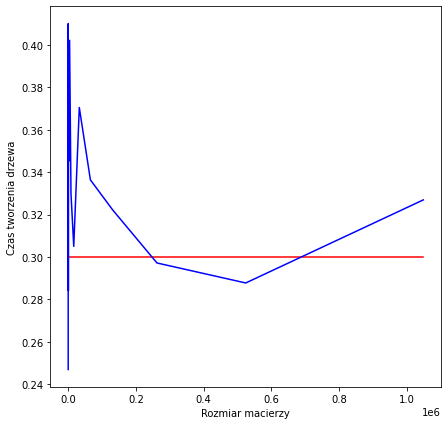
\includegraphics[width=0.6\linewidth]{img/fill01.png}
  \caption{Wykres czasu kompresji od rozmiaru macierzy dla wypełnienia macierzy 10\% z dopasowaną prostą y = 0.3.}
\end{figure}

\begin{figure}[H]
    \captionsetup{justification=centering}
    \centering
  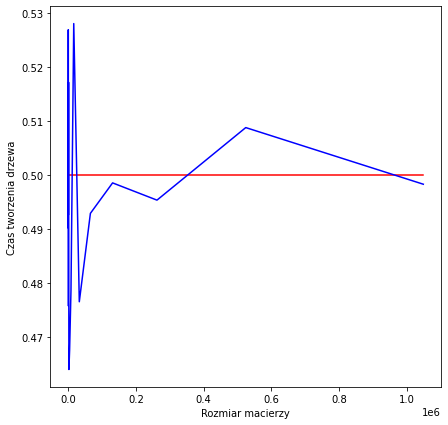
\includegraphics[width=0.6\linewidth]{img/fill02.png}
  \caption{Wykres czasu kompresji od rozmiaru macierzy dla wypełnienia macierzy 20\% z dopasowaną prostą y = 0.5.}
\end{figure}

\begin{figure}[H]
    \captionsetup{justification=centering}
    \centering
  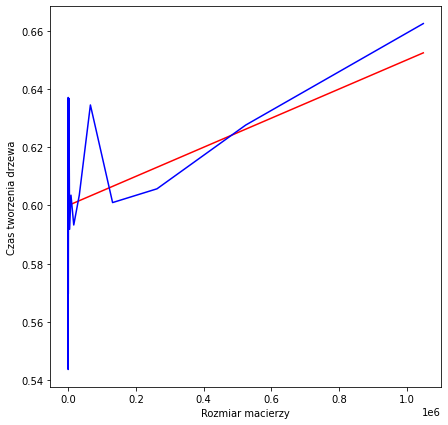
\includegraphics[width=0.6\linewidth]{img/fill03.png}
  \caption{Wykres czasu kompresji od rozmiaru macierzy dla wypełnienia macierzy 30\% z dopasowaną prostą $y = 0.5 * 10^{-7} * x + 0.6$.}
\end{figure}

\begin{figure}[H]
    \captionsetup{justification=centering}
    \centering
  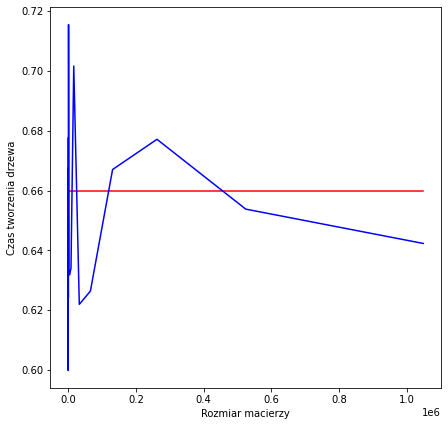
\includegraphics[width=0.6\linewidth]{img/fill04.png}
  \caption{Wykres czasu kompresji od rozmiaru macierzy dla wypełnienia macierzy 40\% z dopasowaną prostą y = 0.66.}
\end{figure}

\begin{figure}[H]
    \captionsetup{justification=centering}
    \centering
  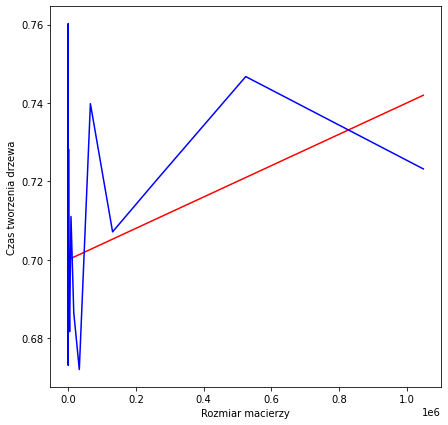
\includegraphics[width=0.6\linewidth]{img/fill05.png}
  \caption{Wykres czasu kompresji od rozmiaru macierzy dla wypełnienia macierzy 50\% z dopasowaną prostą $y = 0.4 * 10^{-7} * x + 0.7$.}
\end{figure}

\subsection{Rysunki}

\begin{figure}[H]
    \captionsetup{justification=centering}
    \centering
  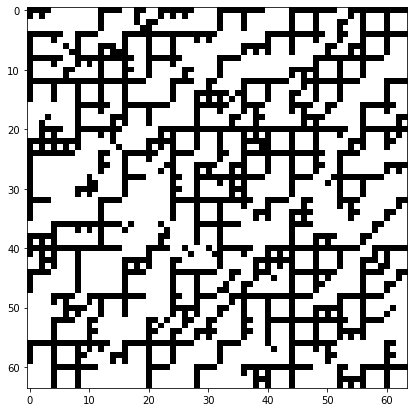
\includegraphics[width=0.6\linewidth]{img/draw01.png}
  \caption{Wizualizacja podziału macierzy dla wypełnienia 10\%.}
\end{figure}

\begin{figure}[H]
    \captionsetup{justification=centering}
    \centering
  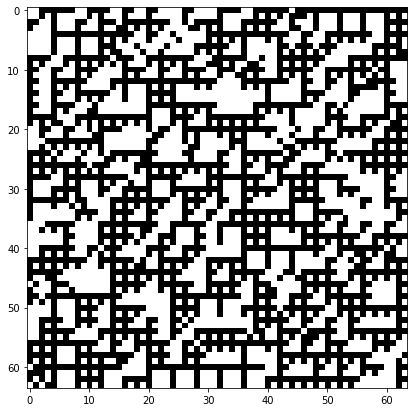
\includegraphics[width=0.6\linewidth]{img/draw02.png}
  \caption{Wizualizacja podziału macierzy dla wypełnienia 20\%.}
\end{figure}

\begin{figure}[H]
    \captionsetup{justification=centering}
    \centering
  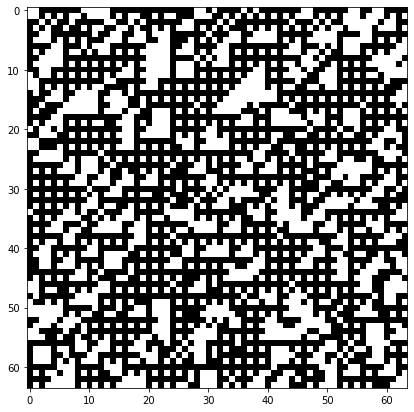
\includegraphics[width=0.6\linewidth]{img/draw03.png}
  \caption{Wizualizacja podziału macierzy dla wypełnienia 30\%.}
\end{figure}

\begin{figure}[H]
    \captionsetup{justification=centering}
    \centering
  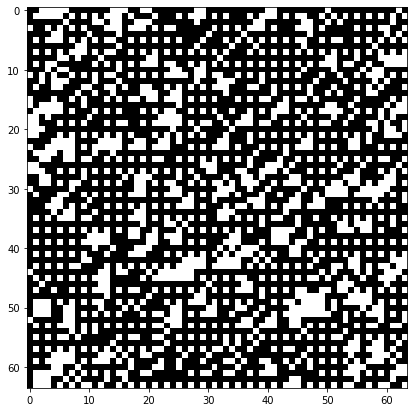
\includegraphics[width=0.6\linewidth]{img/draw04.png}
  \caption{Wizualizacja podziału macierzy dla wypełnienia 40\%.}
\end{figure}

\begin{figure}[H]
    \captionsetup{justification=centering}
    \centering
  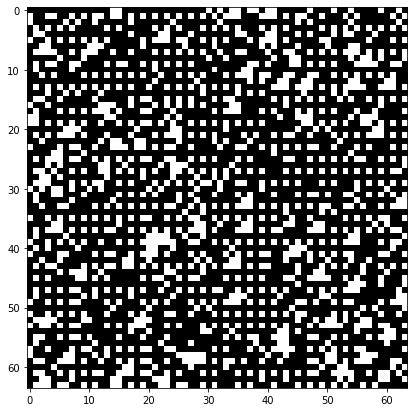
\includegraphics[width=0.6\linewidth]{img/draw05.png}
  \caption{Wizualizacja podziału macierzy dla wypełnienia 50\%.}
\end{figure}

\subsection{Błąd dekompresji}

\begin{table}[H]
\begin{center}
\begin{tabular}{ |c|c|c|c|c|c| } 
    
    \hline
    Wypełnienie & 0.1 & 0.2 & 0.3 & 0.4 & 0.5\\ 
    \hline
    Błąd & bliski 0 & bliski 0 & 0.008 & 0.016 & 0.02 \\ 
    \hline
    
\end{tabular}
\caption{Błąd średniokwadratowy kompresji dla macierzy $128 x 128$}
\end{center}
\end{table}


\end{document}
